\documentclass[aspectratio=169]{beamer}

% ── Theme & Colors ────────────────────────────────────────────────────────────
\usetheme{Madrid}
\usecolortheme{default}

\definecolor{primary}{RGB}{30, 60, 114}
\definecolor{accent}{RGB}{0, 150, 199}
\definecolor{lightgray}{RGB}{245, 245, 248}
\definecolor{successgreen}{RGB}{39, 174, 96}
\definecolor{warnred}{RGB}{192, 57, 43}
\definecolor{warnyellow}{RGB}{241, 196, 15}

\setbeamercolor{palette primary}{bg=primary, fg=white}
\setbeamercolor{palette secondary}{bg=accent, fg=white}
\setbeamercolor{palette tertiary}{bg=primary!80, fg=white}
\setbeamercolor{palette quaternary}{bg=primary, fg=white}
\setbeamercolor{structure}{fg=primary}
\setbeamercolor{section in toc}{fg=primary}
\setbeamercolor{block title}{bg=primary, fg=white}
\setbeamercolor{block body}{bg=lightgray, fg=black}
\setbeamercolor{alertblock title}{bg=warnred, fg=white}
\setbeamercolor{alertblock body}{bg=warnred!10, fg=black}
\setbeamercolor{exampleblock title}{bg=successgreen, fg=white}
\setbeamercolor{exampleblock body}{bg=successgreen!10, fg=black}

% ── Packages ──────────────────────────────────────────────────────────────────
\usepackage[utf8]{inputenc}
\usepackage[T1]{fontenc}
\usepackage[french]{babel}
\usepackage{tikz}
\usetikzlibrary{arrows.meta, positioning, shapes.geometric, fit, backgrounds}
\usepackage{fontawesome5}
\usepackage{booktabs}
\usepackage{array}
\usepackage{xcolor}
\usepackage{graphicx}
\usepackage{hyperref}
\usepackage{grffile}
\usepackage{multimedia}

% ── Metadata ──────────────────────────────────────────────────────────────────
\title[RAG Agentique — Rapport Hebdomadaire]{\textbf{Implémentation du RAG Agentique}\\Rapport d'Avancement Hebdomadaire}
\subtitle{Résultats de Performance, Architecture \& Feuille de Route}
\author[Brahim Bazi \& Youcef El Omari]{\textbf{Brahim Bazi BAZI} \and \textbf{Youcef El Omari EL OMARI}}
\date{\today}


% ── Helpers ───────────────────────────────────────────────────────────────────
\newcommand{\pro}[1]{\textcolor{successgreen}{\faCheckCircle\; #1}}
\newcommand{\con}[1]{\textcolor{warnred}{\faTimesCircle\; #1}}
\newcommand{\todo}[1]{\textcolor{accent}{\faArrowCircleRight\; #1}}
\newcommand{\circled}[1]{\tikz[baseline=(char.base)]{\node[shape=circle,draw,inner sep=1pt] (char) {#1};}}

% ─────────────────────────────────────────────────────────────────────────────
\begin{document}

% ── Title Slide ──────────────────────────────────────────────────────────────
{
\setbeamertemplate{headline}{}
\begin{frame}[plain]
  \vspace{1.2cm}
  \begin{center}
    {\usebeamercolor[fg]{structure}\Huge\textbf{Implémentation du RAG Agentique}}\\[0.3cm]
    {\large\textit{Rapport d'Avancement Hebdomadaire}}\\[0.5cm]
    \rule{8cm}{0.4pt}\\[0.4cm]
    {\large \faUser\ \textbf{Brahim Bazi} \quad\&\quad \faUser\ \textbf{Youcef El Omari}}\\[0.3cm]
    {\small \today}
  \end{center}
  \vfill
  \begin{block}{}
    \centering\small
    Basé sur l'architecture proposée dans \emph{``Developing an AI Assistant for Knowledge Management\\
    and Workforce Training in State DOTs''} — Amaram et al., arXiv:2603.03302v1 (2026)
  \end{block}
\end{frame}
}

% ── Outline ──────────────────────────────────────────────────────────────────
\begin{frame}{Sommaire}
  \tableofcontents
\end{frame}

% ═════════════════════════════════════════════════════════════════════════════
\section{Résultats des Tests de Latence}
% ═════════════════════════════════════════════════════════════════════════════

\begin{frame}{Rappel — Contexte des Tests de Performance}
  \begin{block}{Ce qui restait de la semaine dernière}
    \small
    La semaine dernière, nous avions entamé les tests de performance du pipeline RAG simple mais n'avions pas eu le temps de finaliser l'analyse. Cette semaine, nous présentons les \textbf{résultats complets}.
  \end{block}
  \vspace{0.3cm}
  \begin{columns}[T]
    \begin{column}{0.48\textwidth}
      \begin{exampleblock}{\faFlask\ Protocole Expérimental}
        \small
        \begin{itemize}
          \item \textbf{100 exécutions} (runs) successives du pipeline RAG simple
          \item Même requête et même corpus de documents
          \item Mesures de latence à chaque étape
        \end{itemize}
      \end{exampleblock}
    \end{column}
    \begin{column}{0.48\textwidth}
      \begin{alertblock}{\faCodeBranch\ 3 Approches Comparées}
        \small
        \begin{enumerate}
          \item \textbf{100\% Python} — implémentation classique
          \item \textbf{100\% Rust} — implémentation native
          \item \textbf{Hybride} — orchestration Python + modules critiques en Rust
        \end{enumerate}
      \end{alertblock}
    \end{column}
  \end{columns}
\end{frame}

\begin{frame}{Résultat 1 — Temps Moyen des Embeddings (ms)}
  \begin{columns}
    \begin{column}{0.62\textwidth}
      \centering
      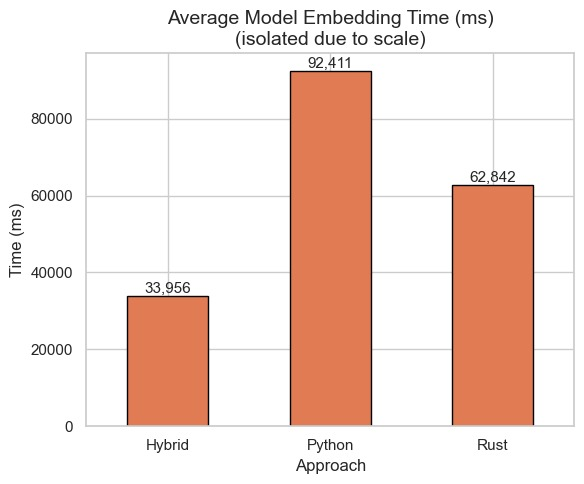
\includegraphics[width=\textwidth,height=0.72\textheight,keepaspectratio]{average_model_embeddings_time_ms.jpg}
    \end{column}
    \begin{column}{0.36\textwidth}
      \begin{block}{Observations}
        \small
        \begin{itemize}
          \item La génération d'embeddings constitue le principal goulot d'étranglement du pipeline.
          \item L'approche \textbf{Hybride} obtient la meilleure latence, combinant l'orchestration Python et les modules Rust optimisés.
          \item \textbf{Rust} arrive en seconde position, et \textbf{Python} reste le plus lent.
        \end{itemize}
      \end{block}
    \end{column}
  \end{columns}
\end{frame}

\begin{frame}{Résultat 2 — Temps d'Exécution du Pipeline (hors embeddings, ms)}
  \begin{columns}
    \begin{column}{0.62\textwidth}
      \centering
      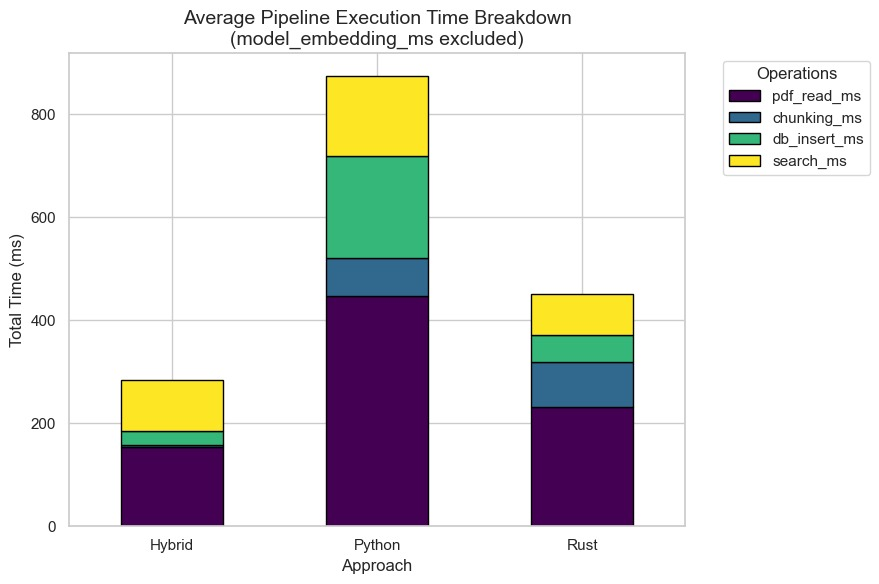
\includegraphics[width=\textwidth,height=0.72\textheight,keepaspectratio]{average_pipeline_execution_time_model_embeddings_ms excluded.jpg}
    \end{column}
    \begin{column}{0.36\textwidth}
      \begin{block}{Observations}
        \small
        \begin{itemize}
          \item En isolant la latence réseau des modèles d'embedding, on mesure le \textbf{coût pur du pipeline RAG} (retrieval + génération).
          \item L'\textbf{Hybride} domine à nouveau avec la latence la plus basse.
          \item \textbf{Rust} suit en deuxième position, \textbf{Python} reste le plus lent.
        \end{itemize}
      \end{block}
    \end{column}
  \end{columns}
\end{frame}

\begin{frame}{Résultat 3 — Tendances sur les 100 Runs}
  \begin{center}
    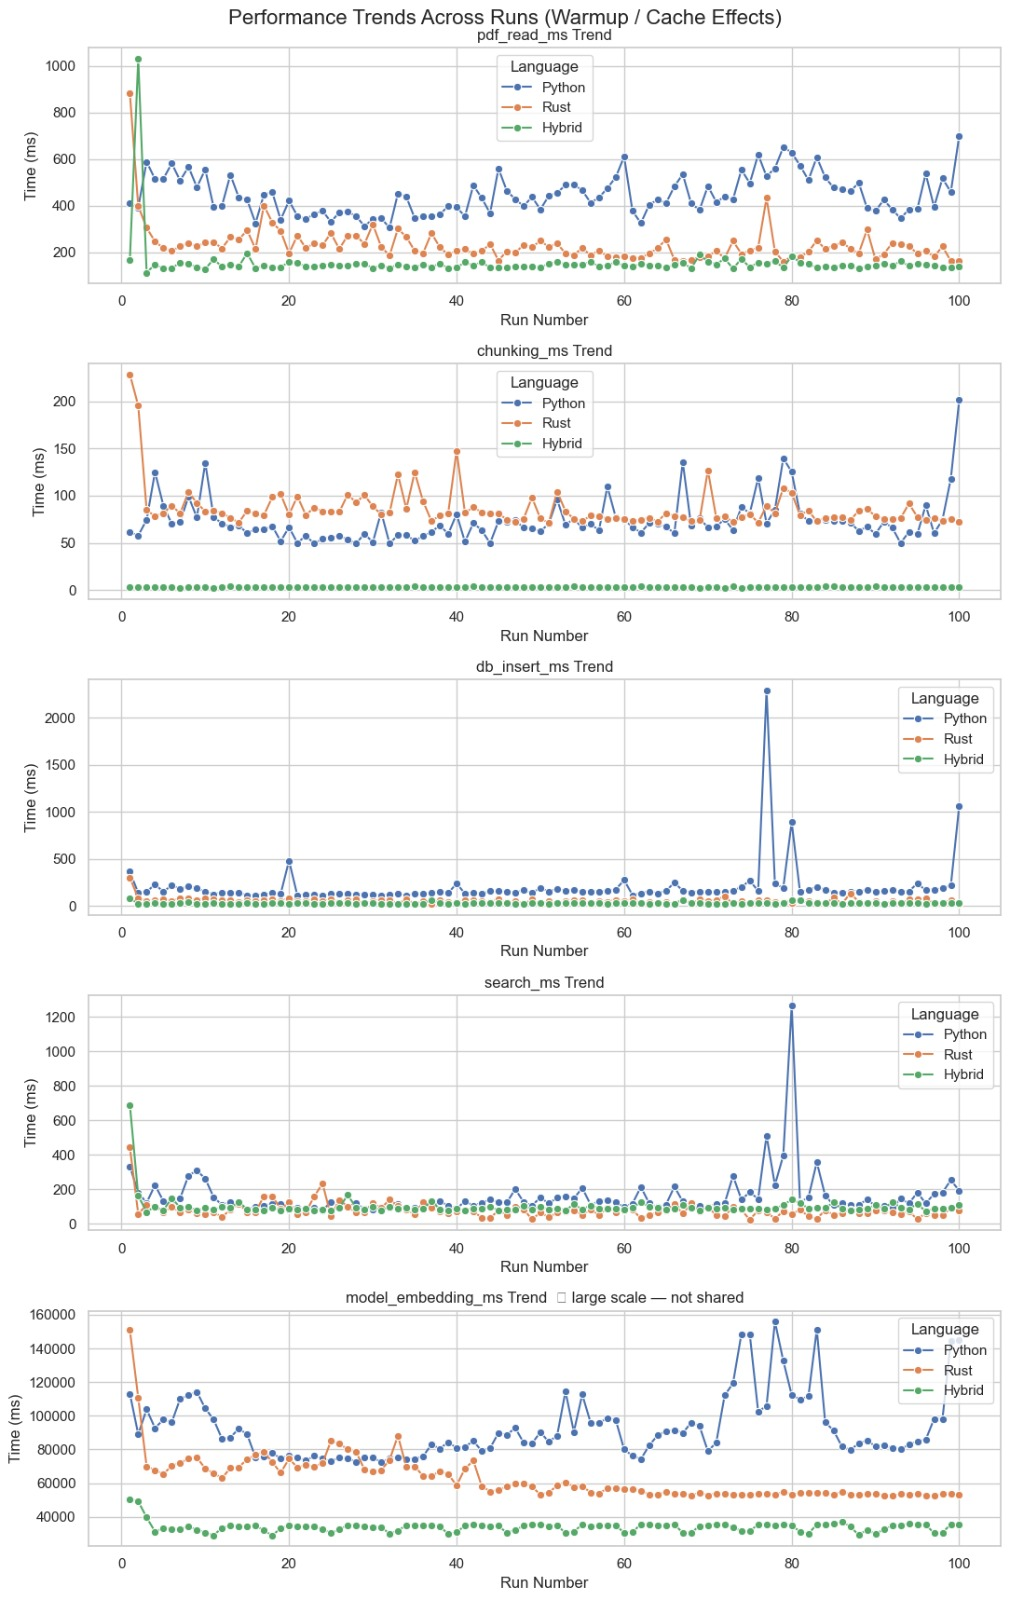
\includegraphics[width=0.52\textwidth,height=0.85\textheight,keepaspectratio]{performance_trends_accross_runs.jpg}
  \end{center}
\end{frame}

\begin{frame}{Analyse — Tendances sur les 100 Runs}
  \begin{block}{Observations}
    \small
    \begin{itemize}
      \item \textbf{Python} présente des pics de latence occasionnels (Garbage Collector, surcharge mémoire).
      \item \textbf{Rust} et \textbf{Hybride} affichent des courbes plus \textbf{stables et prévisibles} au fil des exécutions.
      \item La prévisibilité est cruciale pour un système en production.
    \end{itemize}
  \end{block}
  \vspace{0.3cm}
  \begin{exampleblock}{Conclusion des Tests de Latence}
    \small
    \begin{itemize}
      \item L'approche \textbf{Hybride} (Python + Rust) est la plus performante dans tous les benchmarks — elle combine le meilleur des deux mondes.
      \item L'approche \textbf{100\% Rust} arrive en deuxième position avec de très bonnes performances.
      \item L'approche \textbf{100\% Python} est la plus lente et la moins stable, mais reste la plus simple à développer.
    \end{itemize}
  \end{exampleblock}
\end{frame}

% ═════════════════════════════════════════════════════════════════════════════
\section{Rappel de l'Architecture Multi-Agents}
% ═════════════════════════════════════════════════════════════════════════════

\begin{frame}{L'Architecture RAG Multi-Agents — 5 Agents}
  \begin{center}
  \begin{tikzpicture}[
    node distance=0.7cm and 0.55cm,
    agent/.style={
      rectangle, rounded corners=4pt,
      minimum width=2.1cm, minimum height=0.75cm,
      draw=primary, fill=primary!10,
      font=\small\bfseries, align=center, text=primary
    },
    arrow/.style={-{Stealth[length=5pt]}, thick, color=accent},
    label/.style={font=\scriptsize, color=gray}
  ]
    \node[agent] (user)  {\faUser\\Agent Proxy\\Utilisateur};
    \node[agent, right=of user]  (ret)  {\faSearch\\Agent\\Retriever};
    \node[agent, right=of ret]   (gen)  {\faEdit\\Agent\\Générateur};
    \node[agent, right=of gen]   (eval) {\faCheckSquare\\Agent\\Évaluateur};
    \node[agent, below=0.9cm of eval] (ref)  {\faSyncAlt\\Agent\\Raffineur};

    \draw[arrow] (user) -- node[above, label]{requête} (ret);
    \draw[arrow] (ret)  -- node[above, label]{contexte} (gen);
    \draw[arrow] (gen)  -- node[above, label]{brouillon} (eval);
    \draw[arrow] (eval) -- node[right, label]{feedback} (ref);
    \draw[arrow] (ref.west) -- ++(-0.4,0) |- node[left, label, pos=0.3]{requête raffinée} (ret.south);

    \node[below=0.15cm of user,  font=\tiny, color=gray] {\circled{1}};
    \node[below=0.15cm of ret,   font=\tiny, color=gray] {\circled{2}};
    \node[below=0.15cm of gen,   font=\tiny, color=gray] {\circled{3}};
    \node[below=0.15cm of eval,  font=\tiny, color=gray] {\circled{4}};
    \node[below=0.15cm of ref,   font=\tiny, color=gray] {\circled{5}};

    % Satisfactory exit
    \draw[arrow, color=successgreen] (eval.north) -- ++(0,0.55) node[right, font=\scriptsize, color=successgreen]{\faCheckCircle\ Réponse Finale};
  \end{tikzpicture}
  \end{center}

  \vspace{0.2cm}
  \begin{columns}[T]
    \small
    \begin{column}{0.19\textwidth}
      \textbf{\textcolor{primary}{\circled{1} Proxy}}\\
      Reçoit \& transmet la requête utilisateur
    \end{column}
    \begin{column}{0.19\textwidth}
      \textbf{\textcolor{primary}{\circled{2} Retriever}}\\
      Recherche par similarité dans la base vectorielle
    \end{column}
    \begin{column}{0.19\textwidth}
      \textbf{\textcolor{primary}{\circled{3} Générateur}}\\
      Produit une réponse fondée sur le contexte récupéré
    \end{column}
    \begin{column}{0.19\textwidth}
      \textbf{\textcolor{primary}{\circled{4} Évaluateur}}\\
      Juge la clarté, la pertinence et la complétude
    \end{column}
    \begin{column}{0.19\textwidth}
      \textbf{\textcolor{primary}{\circled{5} Raffineur}}\\
      Reformule la requête si rejeté (max $k$ itérations)
    \end{column}
  \end{columns}
\end{frame}

\begin{frame}{Détails Techniques de l'Implémentation}
  \begin{columns}[T]
    \begin{column}{0.48\textwidth}
      \begin{block}{\faPython\ Stack Utilisé}
        \small
        \begin{itemize}
          \item \textbf{Langage :} Python + modules Rust (via PyO3)
          \item \textbf{LLM :} API OpenRouter (modèles distants)
          \item \textbf{Embeddings :} sentence-transformers
          \item \textbf{Base vectorielle :} LanceDB
          \item \textbf{Ingestion :} Documents texte/PDF
          \item \textbf{API :} FastAPI pour l'interface REST
        \end{itemize}
      \end{block}
    \end{column}
    \begin{column}{0.48\textwidth}
      \begin{exampleblock}{\faCheckCircle\ Ce qui est Fonctionnel}
        \small
        \begin{itemize}
          \item Pipeline complet à 5 agents opérationnel
          \item Boucle de raffinement itérative avec cap
          \item Profilage de performance intégré
          \item Trois variantes (Python / Rust / Hybride) testées et comparées
          \item Déploiement Docker fonctionnel
        \end{itemize}
      \end{exampleblock}
    \end{column}
  \end{columns}
\end{frame}

% ═════════════════════════════════════════════════════════════════════════════
\section{Démonstration}
% ═════════════════════════════════════════════════════════════════════════════

\begin{frame}{Démonstration — Vidéo}
  \begin{center}
    % ── Cliquer sur le cadre pour lancer la vidéo depuis Google Drive ──
    \href{https://drive.google.com/file/d/1rUr8JPeUINm82nMa8qlQ9tejss4O1qVJ/view?usp=sharing}{%
      \begin{tikzpicture}
        \node[minimum width=12cm, minimum height=6.8cm, fill=primary!5, draw=primary, rounded corners=4pt] (vid) {};
        \node at (vid.center) {\textcolor{primary}{\Huge\faPlayCircle}};
        \node[below=0.4cm] at (vid.center) {\textcolor{primary}{\small Cliquer ici pour lancer \texttt{demo.mp4}}};
      \end{tikzpicture}%
    }
  \end{center}
\end{frame}

% ═════════════════════════════════════════════════════════════════════════════
\section{Prochaines Étapes — Semaine Prochaine}
% ═════════════════════════════════════════════════════════════════════════════

\begin{frame}{Ce qu'il Reste à Faire}
  \begin{columns}[T]
    \begin{column}{0.48\textwidth}
      \begin{exampleblock}{\faTasks\ Tâches Prioritaires}
        \small
        \begin{enumerate}
          \item \textbf{Recherche de métriques d'évaluation :} Identifier et implémenter des métriques adaptées aux systèmes RAG agentiques (Faithfulness, Answer Relevancy, Context Precision, Context Recall, etc.)
          \item \textbf{Migration OpenRouter $\to$ Ollama :} Passer d'une API cloud payante à un LLM local via Ollama pour réduire la latence réseau et les coûts
        \end{enumerate}
      \end{exampleblock}
    \end{column}
    \begin{column}{0.48\textwidth}
      \begin{alertblock}{\faBullseye\ Objectifs Secondaires}
        \small
        \begin{itemize}
          \item \textbf{Évaluation avec RAGAS :} Mettre en place un framework d'évaluation automatisé (ex : RAGAS, DeepEval) pour mesurer la qualité des réponses de manière reproductible
          \item \textbf{Enrichissement du corpus :} Tester le système sur un jeu de données plus large et plus représentatif
        \end{itemize}
      \end{alertblock}
    \end{column}
  \end{columns}
\end{frame}

\begin{frame}{Plan d'Action Détaillé}
  \begin{center}
  \renewcommand{\arraystretch}{1.4}
  \small
  \begin{tabular}{>{\bfseries}c l }
    \toprule
    \textbf{\#} & \textbf{Tâche} \\
    \midrule
    1 & Rechercher les métriques d'évaluation pour les RAG \\
    2 & Implémenter les métriques choisies dans le pipeline \\
    3 & Installer et configurer Ollama en local \\
    4 & Migrer les appels LLM d'OpenRouter vers Ollama \\
    5 & Mettre en place RAGAS / DeepEval pour l'évaluation \\
    6 & Explorer la mise en cache des embeddings \\
    \bottomrule
  \end{tabular}
  \end{center}
\end{frame}

% ── Thank You ────────────────────────────────────────────────────────────────
{
\setbeamertemplate{headline}{}
\begin{frame}[plain]
  \vfill
  \begin{center}
    {\Huge\textbf{\textcolor{primary}{Merci}}}\\[0.5cm]
    \rule{6cm}{0.4pt}\\[0.4cm]
    {\large Questions \& Discussion}\\[0.8cm]
    \faUser\ \textbf{Brahim Bazi} \qquad \faUser\ \textbf{Youcef El Omari}
  \end{center}
  \vfill
  \begin{block}{}
    \centering\footnotesize
    Référence : Amaram et al., \textit{``Developing an AI Assistant for Knowledge Management and Workforce Training in State DOTs''}, arXiv:2603.03302v1, February 2026.
  \end{block}
\end{frame}
}

\end{document}
